\documentclass[class=article,border=0pt]{standalone}
\pagestyle{empty}

\usepackage{tikz}
\usepackage{tumcolor}

\begin{document}
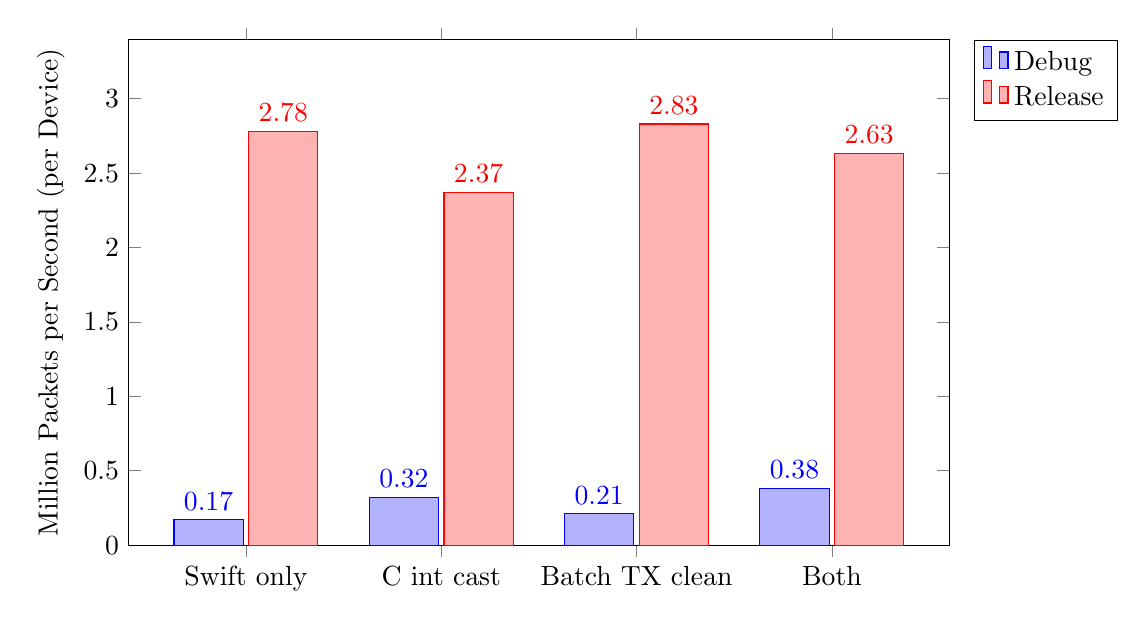
\begin{tikzpicture}
	\begin{axis}[
		ybar,
		ymin=0,
		width=12cm,
		height=8cm,
		bar width=25pt,
		ylabel={Million Packets per Second (per Device)},
		nodes near coords,
		symbolic x coords={Swift only, C int cast, Batch TX clean, Both},
		xtick = data,
		x tick label style={
		/pgf/number format/1000 sep=},
		every node near coord/.append style={
			/pgf/number format/fixed zerofill,
			/pgf/number format/fixed
		},
		legend pos=outer north east,
		legend cell align={left},
		enlarge x limits=0.2,
		enlarge y limits={value=0.2,upper}%,
	]
		\addplot coordinates {(Swift only, 0.17) (C int cast, 0.32) (Batch TX clean, 0.21) (Both, 0.38)};
		\addplot coordinates {(Swift only, 2.78) (C int cast, 2.37) (Batch TX clean, 2.83) (Both, 2.63)};
		\legend{Debug, Release}
	\end{axis}
\end{tikzpicture}

\end{document}
